\section*{General TODOs}

\TODO{QCD has two order parameters:
\begin{enumerate}
\item chiral condensate, incorporated into LSM and NJL, says nothing about confinement!
\item Polyakov loop, not incorporated into LSM and NJL, says something about confinement!
\end{enumerate}
my bag model only contains chiral condensate, so cannot really say much about confinement!
only model this extremely crudely with a bag constant.
more on order parameters: \url{https://physics.stackexchange.com/questions/138255/what-is-an-order-parameter}.
write this in QCD intro and reflect in later chapters.
}

\TODO{front cover: should be A4 (using my extraction script) or slightly bigger correct printing?}
% printing: see
% https://docplayer.me/2690722-Ofte-stilte-sporsmal-trykking-av-masteroppgave-ntnu-grafisk-senter.html,
% https://www.ntnu.no/grafisksenter/studentoppgave

\TODO{title: quark and hybrid stars, not quark stars and hybrid stars}

\TODO{%
	main title suggestion: ``Quark stars and hybrid stars with the quark-meson model'',
	subtitle ``Including detailed introduction to the Tolman-Oppenheimer-Volkoff equation, thermal field theory, ideal neutron stars and stellar stability'' (or only ``compact stars'')
}

\TODO{say that Maxwell construction is almost the same as saying that largest $P$ for given $\mu$ always wins (i.e. lowest and most stable $\Omega$)?}

\TODO{subfigure references are shaky! control this before handing in! fix by regenerating figure to which the reference is wrong.}

\TODO{in figure texts and elsewhere:``quark matter'' sounds like QCD, write quark-meson model matter or something instead} 

\TODO{understand bag-constant as a measure of the trace anomaly? $m = 0$ -- conformal inveriance, classical symmetry broken in the quantum case?}

\TODO{difference between ``perturbative vacuum'' and ``confined vacuum''. ``non-chirally-broken vacuum'' vs ''chirally broken vacuum''? ''confined'' vs ''deconfined'' vacuum?}

\pagebreak

\chapter{Introduction}
\label{chap:master_intro}

\begin{figure}[b]
\centering
\tikzsetnextfilename{stellar-evolution-end}
\begin{tikzpicture}[
	edge from parent/.style={draw,very thick,-latex},
	level distance=5cm,
	level 1/.style={level distance=4.1cm},
	level 2/.style={level distance=3.8cm, sibling distance=6.7cm},
	level 3/.style={level distance=4.7cm},
	level 4/.style={level distance=4.3cm, sibling distance=5.3cm},
	sibling distance=6cm,
	every label/.style={text width=4cm, text centered, inner sep=0pt, yshift=+2pt},
	element/.style={font=\small},
	blackhole/.pic={
		\draw [fill=black, circular glow={fill=red!50!orange}] circle[radius=40pt];
		\draw[draw=none] (-0pt, -55pt) rectangle (+0pt, +55pt);
	},
	neutronstar/.pic={
		\draw[draw=black, fill=blue!  0!purple, circular glow={fill=blue!0!purple}] circle [radius=45pt]; \node [element, rotate=45] at (135:37.5pt) {H}; \node [element] at ( 90:37.5pt) {$\cdots$}; \node [element, rotate=-45] at (45:37.5pt) {Fe};
		\draw[draw=black, fill=blue! 25!purple] circle [radius=30pt]; \node [element, rotate=+45] at (135:22.5pt) {$n$}; \node [element, rotate=0] at (90:22.5pt) {$p$}; \node [element, rotate=-45] at (45:22.5pt) {$e^-$};
		\draw[draw=black, fill=blue! 50!purple] circle [radius=15pt]; \node [element] at (90:0pt) {???};
		\draw[draw=none] (-0pt, -55pt) rectangle (+0pt, +55pt);
	},
	quarkstar/.pic={
		\draw[draw=black, fill=green!50!black, circular glow={fill=green!30!black}] circle [radius=45pt]; \node [element, rotate=0] at (90:32.5pt) {$u$, $d$};
		\draw[draw=black, fill=green!80!black] circle [radius=20pt]; \node [element] at (90:0pt) {$u$, $d$, $s$};
		\draw[draw=none] (-0pt, -55pt) rectangle (+0pt, +55pt);
	},
	whitedwarf/.pic={
		\draw[draw=black, fill=white!80!gray, circular glow={fill=cyan! 20!white}] circle [radius=30pt]; \node [element, rotate=+30] at (120:22.5pt) {H}; \node [element, rotate=-30] at (60:22.5pt) {He};
		\draw[draw=black, fill=cyan!60!white] circle [radius=15pt]; \node [element] at (90:0pt) {C  O};
		\draw[draw=none] (-0pt, -55pt) rectangle (+0pt, +55pt);
	},
]
	\node (whitedwarf) at (0, 0) [label={above:\footnotesize$0.08 M_\odot \lesssim M_0 \lesssim 8 M_\odot$}, label={below:\subcaption{\label{fig:master_intro:star_evolution_white_dwarf}White dwarf}}] {\tikz \pic {whitedwarf};};
	\node (neutronstar) at (3.3, 0) [label={above:\footnotesize$8 M_\odot \lesssim M_0 \lesssim 40 M_\odot$}, label={below:\subcaption{\label{fig:master_intro:star_evolution_neutron_star}Neutron star}}] {\tikz \pic {neutronstar};};
	\node (neutronstar) at (7.5, 0) [label={above:\footnotesize$M_0 \approx 40 M_\odot$ (?)}, label={below:\subcaption{\label{fig:master_intro:star_evolution_quark_star}Quark star (?)}}] {\tikz \pic {quarkstar};};
	\node (blackhole) at (11.5, 0) [label={above:\footnotesize$M_0 \gtrsim 40 M_\odot$}, label={below:\subcaption{\label{fig:master_intro:star_evolution_black_hole}Black hole}}] {\tikz \pic {blackhole};};
\end{tikzpicture}
\caption{\label{fig:master_intro:star_evolution_end}%
	The final stages of a star's life depending on its initial mass $M_0$.
	Between neutron stars and black holes,
	there could be a new class of stars called \textbf{quark stars}.
}
\end{figure}

In \cref{chap:intro} and \cref{fig:intro:star_evolution} we studied how the currently known life cycle of a star
is more or less predetermined by the initial mass $M_0$ of the embryonic \textbf{protostar} born from its parent \textbf{giant molecular cloud}.
Provided that $M_0 \gtrsim 0.08 M_\odot$, the temperature in a protostar reaches the point necessary to ignite fusion of hydrogen, and the star becomes a \textbf{main-sequence star} -- otherwise it retires early as a \textbf{brown dwarf}.
If $0.08 M_\odot \lesssim M_0 \lesssim 8 M_\odot$, a main-sequence star eventually explodes in a \textbf{planetary nebula} and leaves behind a core that collapses under gravity until it stabilizes as a \textbf{white dwarf} (\cref{fig:master_intro:star_evolution_white_dwarf}) supported by the electron degeneracy pressure.
If $8 M_\odot \lesssim M_0 \lesssim 40 M_\odot$, a main-sequence star rather explodes in a \textbf{supernova} and becomes a \textbf{neutron star} (\cref{fig:master_intro:star_evolution_neutron_star}) that is squeezed by gravity beyond the maximum supported pressure of white dwarfs, reaching a new equilibrium mainly supported by the degeneracy pressure of baryons and nuclei.
If $M_0 \gtrsim 40 M_\odot$, the supernova remnant cannot support itself and collapses to a \textbf{black hole} (\cref{fig:master_intro:star_evolution_black_hole}).

\begin{table}
\centering
\begin{tabular}{ l r r l }
	\toprule
	Star & Mass $M$ & Radius $R$ & References \\
	\midrule
	\st{RX J1856.5-3754} & \st{$0.9 M_\odot$} & \st{$\SI{17}{\kilo\meter}$} & \cite{ref:RXJ1856} \\
	3C 58 & unknown & $\SI{15}{\kilo\meter}$ & \cite{ref:3c58} \\
	XTE U1739-285 & $1.5 \, M_\odot$ & $\SI{11}{\kilo\meter}$ & \cite{ref:XTEJ1739} \\
	PSR B0943+10 & $0.02 M_\odot$ & $\SI{2.6}{\kilo\meter}$ & \cite{ref:PSRB0943} \\
	SN1987A remnant & $1.6 M_\odot$ & unknown & \cite{ref:SN1987A_1,ref:SN1987A_2} \\
	ASASSN-15lh & unknown & unknown & \cite{ref:ASASSN} \\
	\bottomrule
\end{tabular}
\caption{\label{tab:master_intro:quark_star_candidates}%
The masses and radii of \st{past} and present quark star candidates.
}
\end{table}

As first proposed by \cite{ref:quark_star_proposition_1}, however,
there could be a narrow range between neutron stars and black holes where a yet unseen equilibrium configuration can be reached,
where the baryons are forced to merge into an ultra-dense form of matter composed of their constituent quarks.
It is speculated that such quark matter can be found in both pure \textbf{quark stars} and inside the cores of \textbf{hybrid neutron stars}.
If quark matter includes strange quarks in addition to up and down quarks, it is referred to as strange quark matter and the star is called a \textbf{strange quark star}.
Although no decisive observation has been made of a quark star,
a few candidates are listed in \cref{tab:master_intro:quark_star_candidates}.
Both their masses and radii are very similar to common neutron stars.

Quarks and the mediators of the strong force between them -- gluons -- are described by the theory of \textbf{quantum chromodynamics}.
Very roughly speaking, it predicts that quarks are confined in hadrons at low temperatures and densities due to a property called \textbf{color confinement},
but deconfined and free of all interactions at high temperatures or densities because of another property called \textbf{asymptotic freedom}.
The confined and deconfined phases are separated by the \textbf{chiral phase transition}.
Unfortunately, it is very hard to work analytically with the general theory of quantum chromodynamics,
so one must turn to approximations and alternative models.
We will model quark stars using the quark-extended linear sigma model, also known as the quark-meson model.

\TODO{add general sources}

\section{Tolman-Oppenheimer-Volkoff equation and stellar stability}
\label{sec:master_intro:tov}

The structure of a spherically symmetric star is governed by the Tolman-Oppenheimer-Volkoff equation
\begin{subequations}
\begin{align}
	\odv{P}{r} &= -\frac{G m \epsilon(P)}{r^2 c^2} \left( 1 + \frac{P}{\epsilon(P)} \right) \left( 1 + \frac{4 \pi r^3 P}{m c^2} \right) \left( 1 - \frac{2 G m}{r c^2} \right)^{-1} , \\
	\odv{m}{r} &= \frac{4 \pi r^2 \epsilon(P)}{c^2} .
\end{align}%
\label{eq:master_intro:tov}%
\end{subequations}%
It is a system of two differential equations for the energy density $\epsilon(r)$, pressure $P(r)$ and mass $m(r)$ as functions of the radius $r$ from the center of the star assumed to be composed of a perfect fluid in hydrostatic equilibrium.
We derived it from the Einstein field equations \eqref{eq:einstein} and studied it in detail in \cref{chap:tov}.
It therefore includes relativistic corrections, which is particularly important for compact stars with extreme density.

To solve it, one must know the fluid's \textbf{equation of state} $\epsilon(P)$ that connects its pressure and energy density, thereby closing the system of three equations and three unknowns.
Then the system can be integrated from the center $r=0$ with zero initial mass $m(0) = 0$ and some central pressure $P(0) = P_c$ until reaching the surface $r=R$ defined by a vanishing pressure $P(R) = 0$.
This yields the radial profiles $\epsilon(r)$, $P(r)$ and $m(r)$, and the total mass $M = m(R)$ can then be calculated.
Thus, one central pressure $P_c$ corresponds to one star with mass $M$ and radius $R$.
As the central pressure is unknown,
it is common to parametrize a sequence of stars with a range of central pressures,
solve the Tolman-Oppenheimer-Volkoff equations for each of them and finally draw a curve of their masses and radii in a mass-radius diagram.

In \cref{sec:nstars:numtov} we wrote a program that integrates the Tolman-Oppenheimer-Volkoff equation for an arbitrary equation of state and generates a smooth mass-radius curve between two given central pressures.
This will be of great use as we encounter new equations of state.

We drew a mass-radius curve for ideal neutron stars in \cref{fig:nstars:massradius}.
Its mass increases with central pressure up to some maximum mass, before decreasing and entering a counterclockwise spiral.
In \cref{sec:nstars:stability_general} we studied the stability of stars along this curve in great detail,
and found that only the stars with lower central pressures than that of the maximum mass star are stable and realized in nature.
This common property of mass-radius curves is the reason that we will focus our attention on the maximum mass and the part of the curve leading up to it.

\section{Thermal field theory in compact stars}
\label{sec:master_intro:tft}

To derive equations of state for quark matter, we will study quantum field theories whose dynamics is described by some Lagrangian density $\lagr$.
In \cref{chap:tft} we showed that the partition function in the grand canonical ensemble corresponding to a Lagrangian including both a fermionic field $\psi$ and a bosonic field $\phi$ is given by the path integral
\begin{equation}
	Z(V, T, \mu_i) = \oint_- \pathintdif \bar{\psi} \oint_- \pathintdif \psi \oint_+ \pathintdif \phi \exp \Big\{ \int_0^\beta \dif \tau \int_V \dif^3 x \, \Big( \lagr_E\big[\bar{\psi}, \psi, \phi\big] + \sum_i \mu_i j^0_i \Big) \Big\} = e^{-\beta V \Omega} .
\label{eq:master_intro:partition_function}
\end{equation}
Here it is the Euclidean Lagrangian density $\lagr_E$ that enters,
obtained from the original Lagrangian $\lagr$ in Minkowski space by substituting an imaginary time variable $t = -i \tau$ into all the fields and then treating $\tau$ as the new ``time'' variable.
The volume of the system is $V$, while its ``temporal'' extent is the system's inverse temperature $\beta = 1/T$.
Sign subscripts are placed on closed path integral signs to remind us of an important property that we showed: bosonic fields must be \emph{periodic} in inverse temperature time, while the fermionic fields must be \emph{anti-periodic}.
We also saw that we could couple any conserved Noether charge densities $j^0_i$ arising from symmetries of the Lagrangian to chemical potentials $\mu_i$.

After computing (the logarithm of) the partition function, it is straightforward to find the grand potential \emph{density}
\begin{equation}
	\Omega(T, \mu_i) = -\frac{\log Z}{\beta V}.
\label{eq:master_intro:grand_potential}
\end{equation}
The volume dependence of the partition function is eliminated by division, turning the extensive quantity $\log Z$ into the intensive quantity $\Omega$.
From the grand potential density, we can calculate the relevant thermodynamic quantities:
\begin{subequations}
\begin{align}
	\text{pressure} \quad P(T, \mu_i) &= -\Omega, \label{eq:master_intro:pressure} \\
	\text{densities} \quad n_i(T, \mu_i) &= -\pdv{\Omega}{\mu_i}, \label{eq:master_intro:densities} \\
	\text{entropy} \quad S(T, \mu_i) &= -\pdv{\Omega}{T} = \beta^2 \pdv{\Omega}{\beta}, \label{eq:master_intro:entropy} \\
	\text{energy density} \quad \epsilon(T, \mu_i) &= \sum_i \mu_i n_i + \pdv{(\beta \Omega)}{\beta} = \sum_i \mu_i n_i - P + T S. \label{eq:master_intro:energy_density}
\end{align}
\end{subequations}
Our goal is to connect a given pressure $P$ to some energy density $\epsilon$ so that we can solve the Tolman-Oppenheimer-Volkoff equation \eqref{eq:master_intro:tov}.
This is greatly simplified in compact stars, where it is common to employ the \textbf{zero-temperature approximation} $T=0$.
We justified this approximation for neutron stars in \cref{sec:nstars:eos} due to the temperature being far lower than the Fermi temperature $T_f$.
With $T = 0$, only the dependence on chemical potentials remain in
\begin{equation}
	P(\mu_i) = -\Omega
	\qquad \text{and} \qquad
	\epsilon(\mu_i) = \sum_i \mu_i n_i - P.
\end{equation}
If there is only one chemical potential $\mu_i = \mu$,
the equation of state $\epsilon(P)$ follows by simply eliminating $\mu$ from $P(\mu)$ and $\epsilon(\mu)$, either numerically or analytically.
This was the case for the neutron star equation of state \eqref{eq:nstars:gr_eos}.
In contrast, the stars we will study now will be composed of up quarks, down quarks, strange quarks and electrons, each associated with a chemical potential.
We then need \emph{three} additional relations to reduce the \emph{four} chemical potentials to \emph{one} independent one, which can then be eliminated to give the equation of state.

\subsection*{Chemical equilibrium of weak interaction processes}

We can obtain two relations between the chemical potentials assuming that the nuclear processes that take place inside the star are in chemical equilibrium.
According to \cite{ref:quark_star_processes}, quarks stars may be formed as hadronic matter in a neutron star decays to strange quark matter through weak interactions processes like
\begin{equation}
u + e^- \rightarrow d + \nu_e
\qquad \text{and} \qquad
u + e^- \rightarrow s + \nu_e .
\end{equation}
As explained in \cite[section 5.3]{ref:glendenning}, neutrinos diffuse out of the star as it cools over time.
We therefore set $\mu_{\nu_e}=0$, so chemical equilibrium of the two processes above implies the two relations
\begin{equation}
\mu_d = \mu_s = \mu_u + \mu_e .
\label{eq:lsm:chemical_equilibrium}
\end{equation}

\subsection*{Electric charge neutrality}

The third and last additional relation relating the four chemical potentials is provided by electric charge neutrality.
We can make a strong and simple classical argument for why there can be no \emph{global} net electric charge in stars by comparing Newton's law of gravity and Coulomb's law of electrostatics.
Suppose a test particle with mass $m$ and electric charge $q$
is placed on the surface $R$ of a spherical star with total mass $M$ and electric charge $Q$.
In an idealized situation where the test particle is affected only by the gravitational and electrostatic force, the total outwards radial force on it is
\begin{equation}
F_\text{out} = -G \frac{M m}{R^2} + k_e \frac{Q q}{R^2} .
\end{equation}
If the star and test particles have opposite charges, $F_\text{out} < 0$ and the particle remains in the star, in a sense seeking to neutralize it.
On the other hand, if the star and particle have like charges, $F_\text{out} > 0$ provided that
\begin{equation}
\frac{Q}{M} > \frac{G}{k_e} \frac{m}{q}.
\end{equation}
In other words, the particle leaves the star and hence seeks to neutralize as long as it is not too heavy.
Even for a heavy baryon like a proton with mass $m = \SI{1.67e-27}{\kilogram}$ and charge $q = +e$ in a common compact star of about one solar mass $M \approx M_\odot$,
\begin{equation}
\frac{Q}{M} \gtrsim 10^{-10} \frac{e}{M_\odot},
\end{equation}
so charged particles will continue to leave the star until it has practically zero electric charge.

In a star that consists of different particle species with charges $q_i$,
we could implement \emph{global} charge neutrality by constraining the chemical potentials $\mu_i(r)$ at every radius $r$ such that the charge density
\begin{equation}
	\sum_p q_p \, n_p(\mu_p(r)) = \rho(r)
\label{eq:intro:charge_neutrality_global}
\end{equation}
integrates to a vanishing total charge $Q = \int_0^R \rho(r) 4 \pi r^2 \dif r = 0$.
This approach would make the equation of state $\epsilon(P)$ at one radius $r$ dependent on its value at \emph{all radii},
and it is not obvious how one should single out one of the infinitely many possible charge density profiles $\rho(r)$.
We will avoid this problem altogether by rather assuming that charge neutrality holds \emph{locally} with $\rho(r) = 0$,
eliminating the chemical potentials at any radius according to
\begin{equation}
	\sum_p q_p \, n_p(\mu_p) = 0
\label{eq:lsm:charge_neutrality}
\end{equation}
The three relations \eqref{eq:lsm:chemical_equilibrium} and \eqref{eq:lsm:charge_neutrality}
reduce the four chemical potentials $\mu_u$, $\mu_d$, $\mu_s$ and $\mu_e$ to one independent chemical potential that can be eliminated from $P(\mu_i)$ and $\epsilon(\mu_i)$ to yield the equation of state $\epsilon(P)$.

As shown in \cite{ref:global_neutrality}, for example, the stronger assumption of local charge neutrality can in fact modify masses and radii of stars within an order of magnitude of solar masses,
but the differences become smaller as one approaches the maximum mass star.
Our choice $\rho(r)=0$ is therefore the simplest choice, but not necessarily the most accurate and physical one.

\section{Quantum chromodynamics}
\label{sec:master_intro:qcd}

\begin{figure}[t]
\centering
%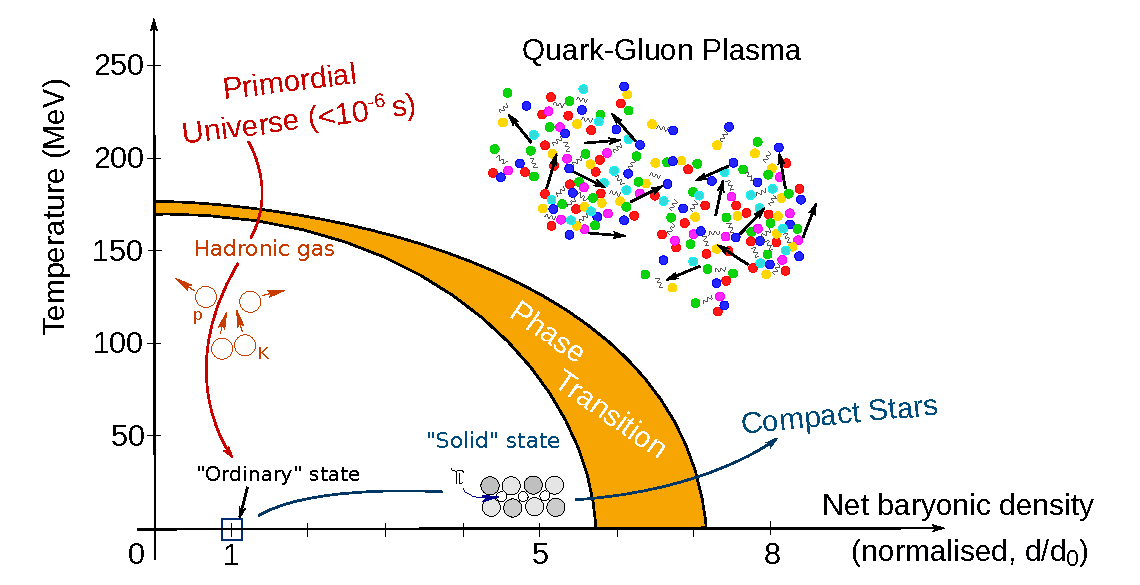
\includegraphics[width=0.9\textwidth]{figures/qcd-phase-diagram.pdf}
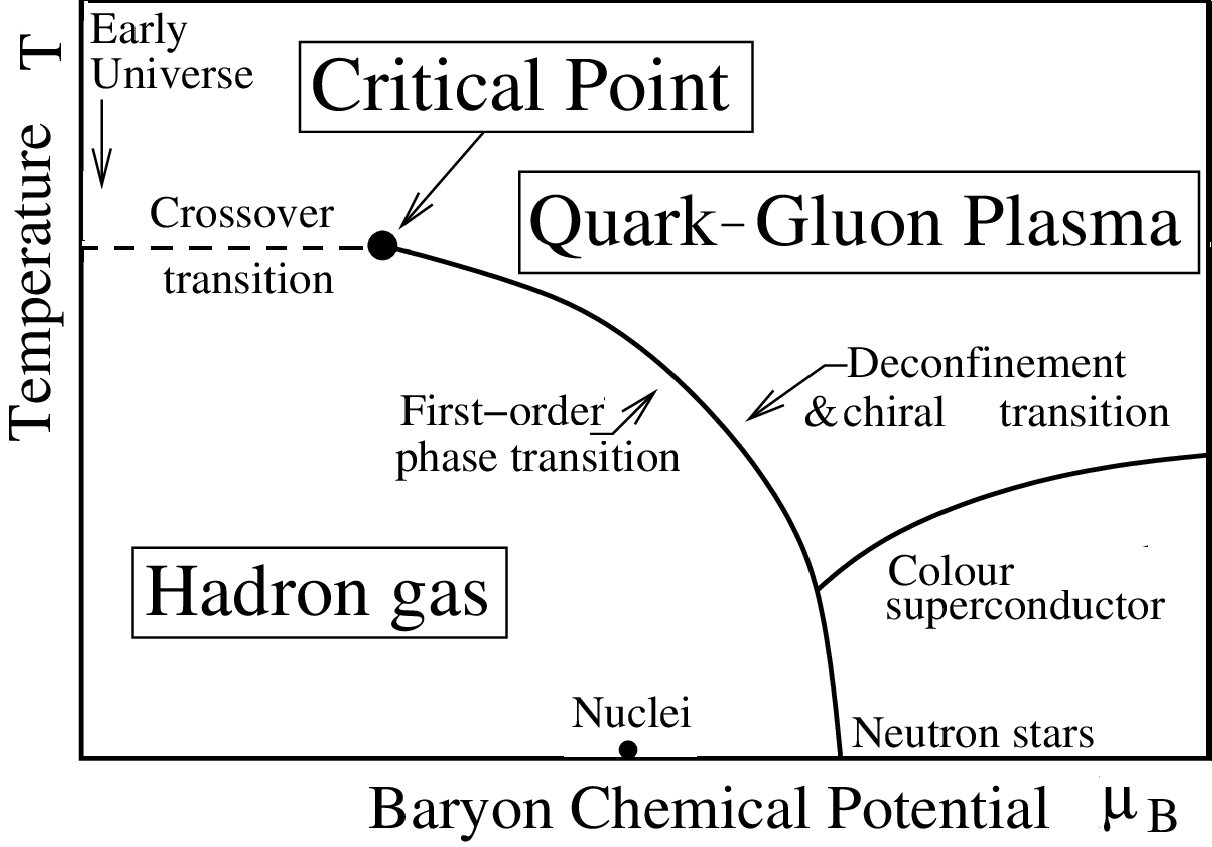
\includegraphics[width=0.6\textwidth]{figures/qcd-phase-diagram.png}
\caption{%
	Slice of the phase diagram of quantum chromodynamics with zero isospin and strangeness.
	%\credit{CERN / Antonin Maire}{https://cds.cern.ch/record/2025215}
	\credit{R.S. Bhalerao}{https://commons.wikimedia.org/wiki/File:PhasDiagQGP.png}
}
\label{fig:qcd:phase_diagram}
\end{figure}
% other phase diagram versions:
% https://en.wikipedia.org/wiki/QCD_matter#/media/File:QCD_phase_diagram.png
% https://en.wikipedia.org/wiki/Quark%E2%80%93gluon_plasma#/media/File:PhasDiagQGP.png
% https://www.researchgate.net/figure/A-sketch-of-the-QCD-Phase-Diagram-according-to-the-collaboration-CBM-at-FAIR-1-it-is_fig1_50218065
% https://cds.cern.ch/record/2729160/plots
% https://physics.aps.org/articles/v3/44
% https://cerncourier.com/a/quark-matter-fireballs-hashed-out-in-protvino/

The theory of the strong interaction force is called \textbf{quantum chromodynamics} (\textbf{QCD}).
It describes the interaction between quarks mediated by gluons through the Lagrangian density
\begin{equation}
	\lagr = \bar{q} ( i \gamma^\mu D_\mu - m ) q - \frac14 G_{\mu\nu}^a G^{\mu\nu}_a
	\qquad \text{with} \qquad
	G_{\mu\nu}^a = \partial_\mu A_\nu^a - \partial_\nu A_\mu^a + g f^{abc} A_\mu^b A_\nu^c.
\label{eq:qcd:lagrangian}
\end{equation}
The quark fields $q = q_{f,c,\alpha}(x)$ are indexed by
the $N_f = 3$ flavors $f \in \{u,d,s\}$,
the $N_c = 3$ colors $c \in \{r,g,b\}$ and
$4$ Dirac spinor indices $\alpha \in \{0,1,2,3\}$,
and we will take a flavor index $f$ with the shorthand $f = q_{f,c,\alpha}(x)$.
The gamma matrices \eqref{eq:tft:gamma_dirac_basis} act in spinor space,
the mass matrix $m = \diag(m_u, m_d, m_s)$ in flavor space,
and there are suppressed identity matrices in spinor, flavor and color space wherever needed for the Lagrangian to be a scalar.
The covariant derivative is $D_\mu = \partial_\mu - i g A_\mu^a T^a$ and couples the gluon gauge fields $A_\mu^a$ to the quarks with strength $g$.
Finally, the Gell-Mann matrices $T^a$ are the $N_a = N_f^2 - 1$ generators of the symmetry group $SU(N_f)$,
whose structure constants $f^{abc}$ can be determined from the commutators $\comm{T^a}{T^b} = i f^{abc} T^c$,
and that are conventionally normalized to $\trace[T^a T^b] = \delta^{ab}/2$.

QCD can be viewed as a generalization of quantum electrodynamics (QED),
where there is a single electron in place of multiple quarks and photons play the role of gluons.
QED is a simpler theory with symmetry group $U(1)$ and is referred to as an \emph{Abelian} gauge theory,
whereas QCD is a \emph{non-Abelian} gauge theory with symmetry group $SU(N_f)$ and an example of a Yang-Mills theory.

\begin{table}[b]
\centering
{ \renewcommand{\arraystretch}{1.2} % restrict scope to this table
\begin{tabular}{ l r r r }
	\toprule
	Quark & Electrical charge & Lone mass & Constituent mass \\
	\midrule
	up ($u$) & $+\frac23 e$ & $\SI{5}{\mega\electronvolt}$ & \approx \, $\SI{300}{\mega\electronvolt}$ \\
	down ($d$) & $-\frac13 e$ & $\SI{7}{\mega\electronvolt}$ & \approx \, $\SI{300}{\mega\electronvolt}$ \\
	strange ($s$) & $-\frac13 e$ & $\SI{150}{\mega\electronvolt}$ & \approx \, $\SI{500}{\mega\electronvolt}$ \\
	\bottomrule
\end{tabular} }
\caption{\label{tab:qcd:quark_properties}%
	Properties of the up, down and strange quarks.
	Lone mass is the mass of a quark by itself \emph{excluding} any gluons,
	while constituent mass refers to the effective mass of a quark in a hadron \emph{including} the surrounding gluon fields.
	The latter can be approximated by the proton and neutron masses $m_p = 2 m_u + m_d \approx m_n = m_u + 2 m_d \approx \SI{900}{\mega\electronvolt}$.
	\cite{ref:pdg_review_2021,ref:glendenning}
}
\end{table}

The main properties of the up, down and strange quarks are gathered in \cref{tab:qcd:quark_properties}.

\subsection*{Phase diagram and calculational methods}
%\label{sec:qcd:phase_diagram_and_methods}

The phase diagram of quantum chromodynamics describes the phase of quark matter
as a function of temperature $T$ and the common quark, isospin and strangeness chemical potentials
\begin{equation}
	\mu   = \frac{\mu_u + \mu_d}{2}, \qquad
	\mu_I = \frac{\mu_u - \mu_d}{2}, \qquad
	\mu_S = \frac{\mu_u - \mu_d}{2} - \mu_s.
\label{eq:master_intro:chemical_potentials_transformed}
\end{equation}
Inverting these relations for the individual quark chemical potentials give
\begin{equation}
	\mu_u = \mu + \mu_I, \qquad
	\mu_d = \mu - \mu_I, \qquad
	\mu_s = \mu - \mu_S .
\label{eq:master_intro:chemical_potentials_particles}
\end{equation}
By the chain rule we can derive that the suitably named common quark chemical potential $\mu$ corresponds to the total quark density
\begin{equation}
	n_Q = -\pdv{\Omega}{\mu} =
	-\pdv{\Omega}{\mu_u} \pdv{\mu_u}{\mu}
	-\pdv{\Omega}{\mu_d} \pdv{\mu_d}{\mu}
	-\pdv{\Omega}{\mu_s} \pdv{\mu_s}{\mu} =
	n_u + n_d + n_s.
\end{equation}
Some authors rather prefer to talk about the baryon chemical potential $\mu_B = 3 \mu$ and baryon density $n_B = n_Q / 3$.
Although mapping out the phase diagram is an active area of research, a rough qualitative picture is known, and the slice with $\mu_I = \mu_S = 0$ is shown in \cref{fig:qcd:phase_diagram}.
We have already argued that one can set $T=0$ in compact stars,
and we will later see that the additional constraints of chemical equilibrium \eqref{eq:lsm:chemical_equilibrium} and charge neutrality \eqref{eq:lsm:charge_neutrality} entail that
the state of quark matter in compact stars is parametrized by a curve in the diagram that lies close to the $\mu$-axis.
We will shortly discuss the most important qualitative properties of quantum chromodynamics and relate them to this phase diagram.

The general theory of quantum chromodynamics is notorious for being very difficult to work with,
and its elegance and practicality stops not longer after writing down its Lagrangian \eqref{eq:qcd:lagrangian}.
To explore the phase diagram, one must therefore turn to alternative techniques:
\begin{itemize}
\item \textbf{Perturbation theory} can be used to study quantum chromodynamics analytically at \emph{high} energy, perhaps contrary to what one might expect.
      As we will soon discuss in more detail, this is due to a property called asymptotic freedom that causes the interaction strength to \emph{decrease} with increasing energy.
\item \textbf{Lattice QCD} consists of making numerical calculations on a discrete lattice of spacetime points.
      This method has proved very useful for studying quantum chromodynamics under quite general circumstances.
      In the regime of high baryon density and low temperature, however, is plagued by the so-called sign problem that refers to the difficulty of calculating integrals of highly oscillatory functions.
      This is precisely the region of the phase diagram that is relevant for compact stars.
\item The \textbf{$\bm{1/N_c}$-approximation} or \textbf{large $\bm{N_c}$-limit} consists of making expansions in the assumed small parameter $1/N_c$.
      Although there are only $N_c = 3$ colors in nature, this scheme has indeed been used to make accurate predictions.
      We will refer to this approximation to justify some of our later actions.
\item \textbf{Effective theories and models} can be used to study quantum chromodynamics in some regimes of interest.
      The most important requirements of such a theory or model is that it includes the correct degrees of freedom (or particles) and exhibits the same symmetries and symmetry breaking patterns as the theory it aims to describe in the targeted regime.
      Due to \cite{ref:weinberg_eft}, the philosophy is then to ``write down the most general possible theory involving fields for these particles, including all possible interactions consistent with the symmetries''.
      Chiral perturbation theory ($\chi$PT) is an example of an effective low-energy theory obtained systematically in this way,
      and the Nambu-Jona-Lasinio (NJL) model and the quark-extended linear sigma model (LSM), also known as the quark-meson (QM) model, are effective models in the same regime.
      This approach is applicable to compact stars and is the one we will take.
      \TODO{separate $\chi$PT from NJL/LSM. good now?}
\end{itemize}

\subsection*{Color confinement and asymptotic freedom}

\TODO{inspiration: \cite{ref:quark_bag_model} and more?}

\begin{figure}[t]
\centering
\tikzsetnextfilename{colorless-hadrons}
\colorlet{rgbcyan}[rgb]{cyan}
\colorlet{rgbmagenta}[rgb]{magenta}
\colorlet{rgbyellow}[rgb]{yellow}
%\definecolor{rgbcyan}{cmyk}{1,0,0,0}
%\definecolor{rgbmagenta}{cmyk}{0,1,0,0}
%\definecolor{rgbyellow}{cmyk}{0,0,1,0}
\begin{tikzpicture}
\node (meson) { \tikz {
	\begin{scope}[blend group=screen]
		\draw [draw=black, fill=rgbcyan]  (30:1.0)  circle (1.50);
		\draw [draw=black, fill=red] (150:1.0) circle (1.50);
	\end{scope}
} };
\node (baryon) [right=of meson, xshift=+4.0cm] at (0, 0) { \tikz {
	\begin{scope}[blend group=screen]
		\draw [draw=black, fill=red]   (30:1.0)  circle (1.50);
		\draw [draw=black, fill=green] (150:1.0) circle (1.50);
		\draw [draw=black, fill=blue]  (270:1.0) circle (1.50);
	\end{scope}
} };
\end{tikzpicture}
\caption{\label{fig:qcd:colorless_hadrons}%
	A ``white'' meson composed of a \textcolor{red}{red} and \textcolor{cyan}{antired} quark and
	a ``white'' baryon composed of a \textcolor{red}{red}, \textcolor{blue}{blue} and \textcolor{green}{green} quark.
}
\end{figure}

One fundamental feature of quantum chromodynamics is \textbf{color confinement}.
Quarks can be color-charged \textcolor{red}{\textbf{red}}, \textcolor{green}{\textbf{green}} and \textcolor{blue}{\textbf{blue}},
while antiquarks can have the complementary anticolors \textcolor{cyan}{\textbf{antired}}, \textcolor{magenta}{\textbf{antigreen}} and \textcolor{yellow}{\textbf{antiblue}}.
At low temperature and density, experiments and lattice simulations show that quarks never appear in isolation, but are always confined in hadrons that have no overall color.
As the distance between color-charged quarks increases, the strong force between them remains \emph{constant} -- the quarks are  effectively ``glued'' together by mediating gluons.
For example, a meson consists of one quark of any color and one antiquark of its complementary color, making the meson itself colorless or ``white''.
Similarly, a(n) (anti)baryon consists of one (anti)red, one (anti)green and one (anti)blue quark and is also ``white''.
Such ``white'' bound states illustrated in \cref{fig:qcd:colorless_hadrons} are also referred to as \textbf{color singlets}.

What if an even stronger force overcomes the strong force and tries to forcibly separate the quarks in a hadron into colorful groups of quarks?
Then nature will simply create new quark--anti-quark pairs so that the new groups of quarks both become new colorless hadrons.
At low temperatures and densities in the lower left of \cref{fig:qcd:phase_diagram}, quarks are therefore always \emph{confined} in colorless hadronic matter that make up the present world around us.

In the opposite extreme of high temperature or density in \cref{fig:qcd:phase_diagram}, quantum chromodynamics displays the property of \textbf{asymptotic freedom}.
As the energy scale of quark interactions increases, or equivalently its length scale decreases, the interaction strength \emph{decreases} and quarks become \emph{deconfined}.
With increasing temperature, experiments and calculations have shown that the deconfined phase is a \textbf{quark-gluon plasma} of free color charges and gluons.
It is believed that the universe passed through this phase during the first $\SI{20}{\micro\second}$ after the Big Bang, after which it transitioned to the present phase of hadronic matter.
The situation with low temperature and increasing baryon density is more uncertain:
no human-made laboratory can recreate the extreme densities required for quark matter,
and calculations are difficult and suggest qualitative features that depend on the model used.
Only in the extreme limit of infinite baryon density, where perturbation theory applies,
it is known that the deconfined phase turns into a \textbf{color-flavor-locked phase} of superconducted \TODO{superconducting?} color charges.
Asymptotic freedom was first discovered by \cite{ref:asymptotic_freedom_gross_wilczek,ref:asymptotic_freedom_politzer}, who were recognized with the Nobel Prize in 2004.
\TODO{få Jens til å ``godkjenne''}

%As the temperature increases, confined hadronic quark matter turns into a \emph{deconfined} \textbf{quark-gluon plasma} in the upper right of \cref{fig:qcd:phase_diagram} where they are free of all interactions and move around at will.
%It is believed that the universe passed through this phase during the first $\SI{20}{\micro\second}$ after the Big Bang, after which it transitioned to the present phase of hadronic matter.
%As no human-made laboratory can possibly recreate the necessary densities in the near future, the best candidates for finding and studying this exotic state of matter today is precisely the cores of compact stars.
%Asymptotic freedom was first discovered by \cite{ref:asymptotic_freedom_gross_wilczek,ref:asymptotic_freedom_politzer}, who were recognized with the Nobel Prize in 2004.
%\TODO{third superconducting phase, situation is not so black--white}

\subsection*{Vector, axial and chiral symmetries and chiral symmetry breaking}
%\label{sec:qcd:symmetry}

The Lagrangian \eqref{eq:qcd:lagrangian} has some interesting global symmetries, each of which gives rise to a conserved classical current by Noether's theorem.
The simplest symmetry is the $U(1)_V$ \textbf{vector symmetry} $q \rightarrow e^{i \theta} q$, giving rise to the conserved vector current $j^\mu = \bar{q} \gamma^\mu q$ representing the baryon number density.
In the grand canonical ensemble, we will later couple one such conserved current to a chemical potential for each quark flavor.
In the massless case $m = 0$, the Lagrangian also has the $U(1)_A$ \textbf{axial symmetry} $q \rightarrow e^{i \theta \gamma^5} q$ with the conserved axial current $j^\mu = \bar{q} \gamma^\mu \gamma^5 q$.
As its proof assumes the action to be extremized, Noether's theorem is inherently \emph{classical}.
Unlike the vector current, the axial current is no longer conserved under the influence of quantum effects, and is therefore said to be \emph{anomalous}.

Using the projection operator $P_\pm = \frac12 (1 \pm \gamma^5)$, we can introduce the left-handed ($-$) and right-handed ($+$) chiral fields $q_\pm = P_\pm q$.
One can then show that $q = q_- + q_+$, $\bar{q}_\pm q_\pm = 0$ and $\bar{q}_\pm \gamma^\mu D_\mu q_\mp = 0$, so that the Lagrangian \eqref{eq:qcd:lagrangian} can be written
\begin{equation}
	\lagr = \bar{q}_- i \gamma^\mu D_\mu q_- + \bar{q}_+ i \gamma^\mu D_\mu q_+ - \bar{q}_- m q_+ - \bar{q}_+ m q_- - \frac14 G_{\mu\nu}^a G^{\mu\nu}_a.
\label{eq:qcd:lagrangian_chiral}
\end{equation}
In the massless case $m=0$,
it is left invariant under the $SU(N_f)_L \times SU(N_f)_R$ \textbf{chiral symmetry} transformation $q_\pm \rightarrow U_\pm q_\pm$ where both $U_\pm \in SU(N_f)$.
Moreover, it is known that the ground state of quantum chromodynamics admits a nonzero quark condensate \cite[chapter 28]{ref:schwartz}
\begin{equation}
	\avg{\bar{q} q} %= \avg{\bar{q}_- q_-} + \avg{\bar{q}_+ q_+} + \avg{\bar{q}_- q_+} + \avg{\bar{q}_+ q_-}
	                                                            = \avg{\bar{q}_- q_+} + \avg{\bar{q}_+ q_-},
\end{equation}
which is generally \emph{not} invariant under the chiral transformation.
The fact that the ground state does not carry the same symmetry as its Lagrangian is the signature of \textbf{spontaneous symmetry breaking}.
Only if $U_- = U_+$ are all terms invariant -- this is the $SU(N_f)_V$ \textbf{vector symmetry} where both left-handed and right-handed fields are transformed in the same way.
The isospin symmetry is also a symmetry of the \emph{massive} Lagrangian \eqref{eq:qcd:lagrangian_chiral} \emph{if} all quark masses are set equal so that the mass matrix $m$ is proportional to the identity matrix.
We therefore say that quantum chromodynamics exhibits \textbf{chiral symmetry breaking}
\begin{equation}
	SU(N_f)_L \times SU(N_f)_R \quad (m = 0) \qquad \longrightarrow \qquad SU(N_f)_V \quad (m \neq 0).
\label{eq:qcd:symmetry_breaking_pattern}
\end{equation}
Goldstone's theorem then predicts that one massless Goldstone boson arises from every broken symmetry generator.
Hence, chiral symmetry breaking gives rise to $2 \times (N_f^2 - 1) - (N_f^2 - 1) = N_f^2 - 1$ Goldstone bosons.
With $N_f = 2$ and $N_f = 3$ flavors, these are the three pions and the eight scalar mesons.

In the real world, however, the quarks have different masses and cause the chiral symmetry to be only \emph{approximately} broken.
We say that the different quark masses cause \textbf{explicit symmetry breaking}, in the sense that the Lagrangian changes by a small amount under the chiral transformation.
The physical consequence of this is that there are no massless Goldstone bosons, but rather very light pseudo-Goldstone bosons.

The breaking of chiral symmetry leads to the \textbf{chiral phase transition} shown in \cref{fig:qcd:phase_diagram},
connecting the confined and deconfined phases of quark matter.
\TODO{%
round off with magnet analogy (see JO book for details).
adding $B$ explicitly breaks symmetry and essentially generates massive ``quarks'':
\begin{itemize}
\item quark masses are like external magnetic field (that cause ESB instead of SSB)
\item chiral condensate is like magnetization
\end{itemize}
}
